% This include all the settings that we should use for the document
\newcommand{\UPPDFTitle}{Altera University Program Flash Memory IP Core}
\newcommand{\UPTextBar}{SOPC Builder and Standalone IP Core}
\newcommand{\UPTemplatePath}{U:/Internal/Templates}
\input{\UPTemplatePath/Docs/defaulttext.tex}
\input{\UPTemplatePath/Docs/preamble.tex}

%%%%%%%%%%%%%%%%%%%%%%%%%
% Add title
%%%%%%%%%%%%%%%%%%%%%%%%%
% Add title
\newcommand{\doctitle}{Altera University Program \\ Flash Memory IP Core}
\newcommand{\dochead}{Flash Memory IP Core for Altera DE Boards}
% Usually no need to change these two lines
\title{\fontfamily{phv}\selectfont{\doctitle} }
\chead{ \small{\textsc{\bfseries \dochead} } }
% Customizations
%%%%%%%%%%%%%%%%%%%%%%%%%

\begin{document}
\begin{table}[h]
    \centering
    \begin{tabular}{p{5cm}p{4cm}}
        \hspace{-3.5cm}\includegraphics[width=0.4\textwidth]{\UPTemplatePath/Figures/Altera.pdf}
        &
        \raisebox{1\height}{\parbox[h]{0.4\textwidth}{\Large\fontfamily{phv}\selectfont{\textbf{\doctitle}}}}
    \end{tabular}
    \label{tab:logo}
\end{table}

\colorbox[rgb]{0,0.384,0.816}{\parbox[h]{\textwidth}{\color{white}\textbf{\textit{\UPTextBar}}}}

\thispagestyle{plain}

\section{Core Overview}
%    * Describe the function of the core, from a system-level perspective, at a very high level.
%    * Explain why this component exists. What type of problem was the core created to solve?
%    * List major features of the core.
%    * List approximate resource usage & performance for a basic configuration
%    (if appropriate). Note that if the size of the core differs wildly,
%    depending on the configuration, it's better to not set expectations one
%    way or the other. Or, state a range, and make it clear that "your mileage
%    will vary."
%    * Note significant differences from other similar cores (if applicable).
A Flash Memory is a non-volatile type of memory that can be electrically erased and reprogrammed. It is similar
to volatile types of memory, such as SRAM and DRAM, in that it can be written to and read; however, it is different
in that it retains its data even when the memory device is powered down. The ability to retain its data makes it useful in
applications such as Secure Data cards and USB memory sticks for the purposes of storing and transporting data.

While flash memory is versatile it has its limitations. Unlike volatile memory, to change the memory contents
the data present in the memory must first be erased and only then can new data be written. The underlying technology also
places a limitation on the number of times data can be written reliably to any particular location of the flash memory. Typically,
flash memory devices allow each memory location to be written in the order of 10000 times, and up to 100000 in high-end
parts.

The Altera University Program (UP) Flash Memory IP Core is a hardware component that facilitates the use of flash memory devices
present on the Altera DE1 and DE2 boards. We provide this core for general use, however we advise that the flash memory
not be used for temporary data storage, as doing so may significantly reduce the lifetime of
the flash memory chips.

This document describes how to instantiate the Altera UP Flash Memory IP Core in an
System-on-Programmable-Chip (SOPC) Builder based design as well as a standalone module in user designs.

\section{Functional Description}
%    *  This section describes the hardware structure of the core, and how it functions.
%    * Show a block diagram of the core. For cores that vary in shape depending
%    on parameters, you might have to show a typical or a maximal
%    configuration. List the input and output signals of the core.
%    * Describe each functional unit of the core hardware.
%    * If possible, include a high-level narrative of how the core operates in
%    a system. I.e., "Data comes from point A. The core processes it in
%    functional unit B. The core sends processed data out to point C." Each
%    functional unit of the core can contain some narrative about how it
%    behaves in a system.

The Altera UP Flash Memory IP Core is supplied with two interfaces: a standalone interface, and Avalon Interconnect Interface. The standalone interface is
intended for use in designs where an Avalon Interconnect is not used. The Avalon Interconnect Interface should be used in SOPC Builder based systems, where the core will become a memory mapped I/O slave attached to the Avalon Interconnect. We describe the functionality of both versions of the core in the following subsections.

\subsection{Standalone Version}

\begin{figure}[h]
\centering
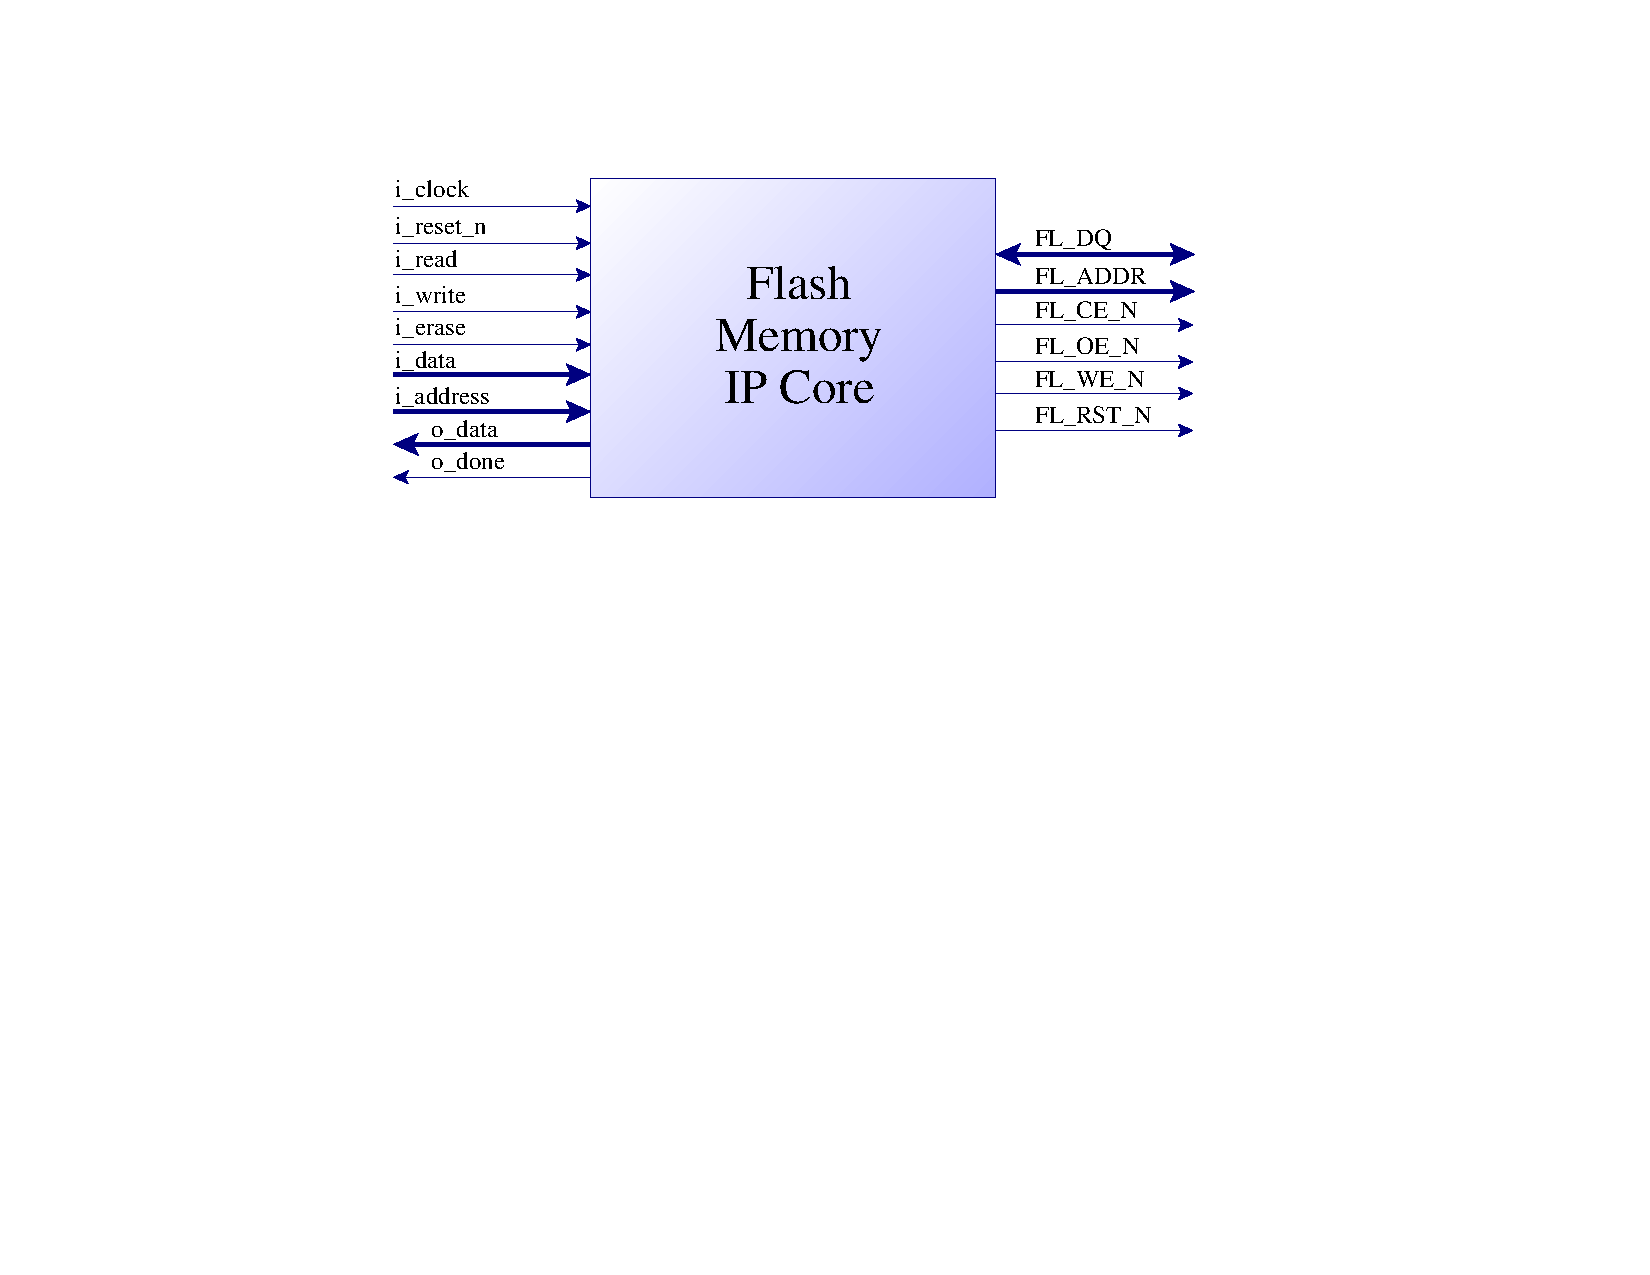
\includegraphics[width=3.5in,,,clip=false]{fig_flash_standalone.pdf}
\caption{Standalone Flash Memory IP Core Interface.}\label{fig:standalone}
\end{figure}
The standalone interface diagram of the Altera UP Flash Memory IP Core is shown in Figure~\ref{fig:standalone}. It consists of user interface signals on the left-hand side, and a flash memory chip signals on the right-hand side. The signals on the left-hand side are all single bit wires, with the exception of {\it i\_data}, {\it o\_data}, and {\it i\_address}. The data ports are both 8 bit wide, while the input address is defined by a {\it FLASH\_MEMORY\_ADDRESS\_WIDTH} parameter. By default, the flash memory address width parameter is set to 22, indicating that 22 address bits are necessary to address each byte in a 4MB flash memory device. The remaining signals on the left-hand side are control signals that allow the flash memory to be read, written and erased.

The flash memory chip signals shown on the right hand side connect to the flash memory device on a DE board. Port {\it FL\_DQ} is an 8-bit bidirectional bus that carries the data to and from the flash memory device. The address in the memory to be accessed is specified by the {\it FL\_ADDR} output port. Its width matches that specified by {\it FLASH\_MEMORY\_ADDRESS\_WIDTH} parameter. The other output signals are 1-bit wide each, and control data transfer between the Flash Memory IP Core and the flash memory device.

In the following subsections we describe how each set of signals operates.

\subsubsection{User Interface}

In addition to data and address lines described earlier, the user interface inputs include an {\it active-low} asynchronous reset, {\it i\_reset\_n}, a clock input called {\it i\_clock}, as well as control signals {\it i\_read}, {\it i\_write}, {\it i\_erase}, and {\it o\_done}. The asynchronous reset signal will reset the internal FSM to an initial state, where the circuit will reset the flash memory device and prepare it for data exchange. The clock signal should connect to a 50MHz clock signal.

To transfer data between to and from the flash memory, several control signals are provided. The {\it i\_read} signal causes the circuit to read a byte of data specified by the {\it i\_address} input and produce it at the {\it o\_data} output. Please note that the output will only be valid when the {\it o\_done} signal is raised. Thus, the {\it i\_read} signal should remain high until {\it o\_done} is raised, before the data from the {\it o\_data} lines is read. The {\it i\_write} signal functions in a similar manner. When high, the {\it i\_write} signal causes data at input {\it i\_data} to be written at the address specified by {\it i\_address}. The operation completes when {\it o\_done} is raised. Please note that no other operation can be performed while a read/write operation is ongoing.

The {\it i\_erase} signal functions differently. When {\it i\_erase} is raised high, it causes a sector of memory to be erased. The sector that will be erased is the one which contains the byte at address specified by the {\it i\_address} input. The only exception is when the {\it i\_address} input consists of all 1s. In such a case, the entire flash memory device will be erased. It is important to note that the erase operation is critical to the proper operation of the flash memory. To write new data to an occupied memory location, it is necessary to erase the specified memory location first. This results in a hexadecimal value {\bf FF} to be stored in the erased memory locations. Once the memory, either a sector of 8k/64k bytes or the entire chip, has been erased, the {\it o\_done} signal will be raised.
Please note that no other operations can be performed while an erase operation is ongoing.

Most flash memory interfaces allow data writes to previously written locations without forcing an erase operation to be executed first. Doing so is inadvisable, because the new data cannot be guaranteed to be stored correctly. More specifically, any bit that has been set to 0 cannot be changed to a 1 without using the memory location first. To protect the flash memory devices from accidental misuse, the Altera UP Flash Memory IP Core includes a protection mechanism that prevents writing data to non-empty memory locations. Any attempt to do so will result in the circuit behaving as though the operation succeeded. However, no data will actually be written to the specified memory location. A subsequent read operation will show that the memory contents remain unchanged.

\subsubsection{Flash Memory Chip Interface}

The signal connected to the flash memory device directly include {\it FL\_DQ}, {\it FL\_ADDR}, {\it FL\_OE\_N}, {\it FL\_WE\_N}, {\it FL\_CE\_N}, and {\it FL\_RST\_N}. The {\it FL\_DQ} is a set of 8 bidirectional wires used to transfer data between the IP Core and the flash memory chip. The address of the data to be accessed is specified by the {\it FL\_ADDR} lines. The remaining ports are control signals that ensure the transfer of data is completed correctly. The detailed behaviour of these signals is beyond the scope of this document. Further details on this topic can be found in the datasheet for the given flash memory device. 

\subsection{SOPC Builder Version}

The SOPC Builder version of the flash memory IP core is shown in Figure~\ref{fig:avalon_interface}.

\begin{figure}[h]
\centering
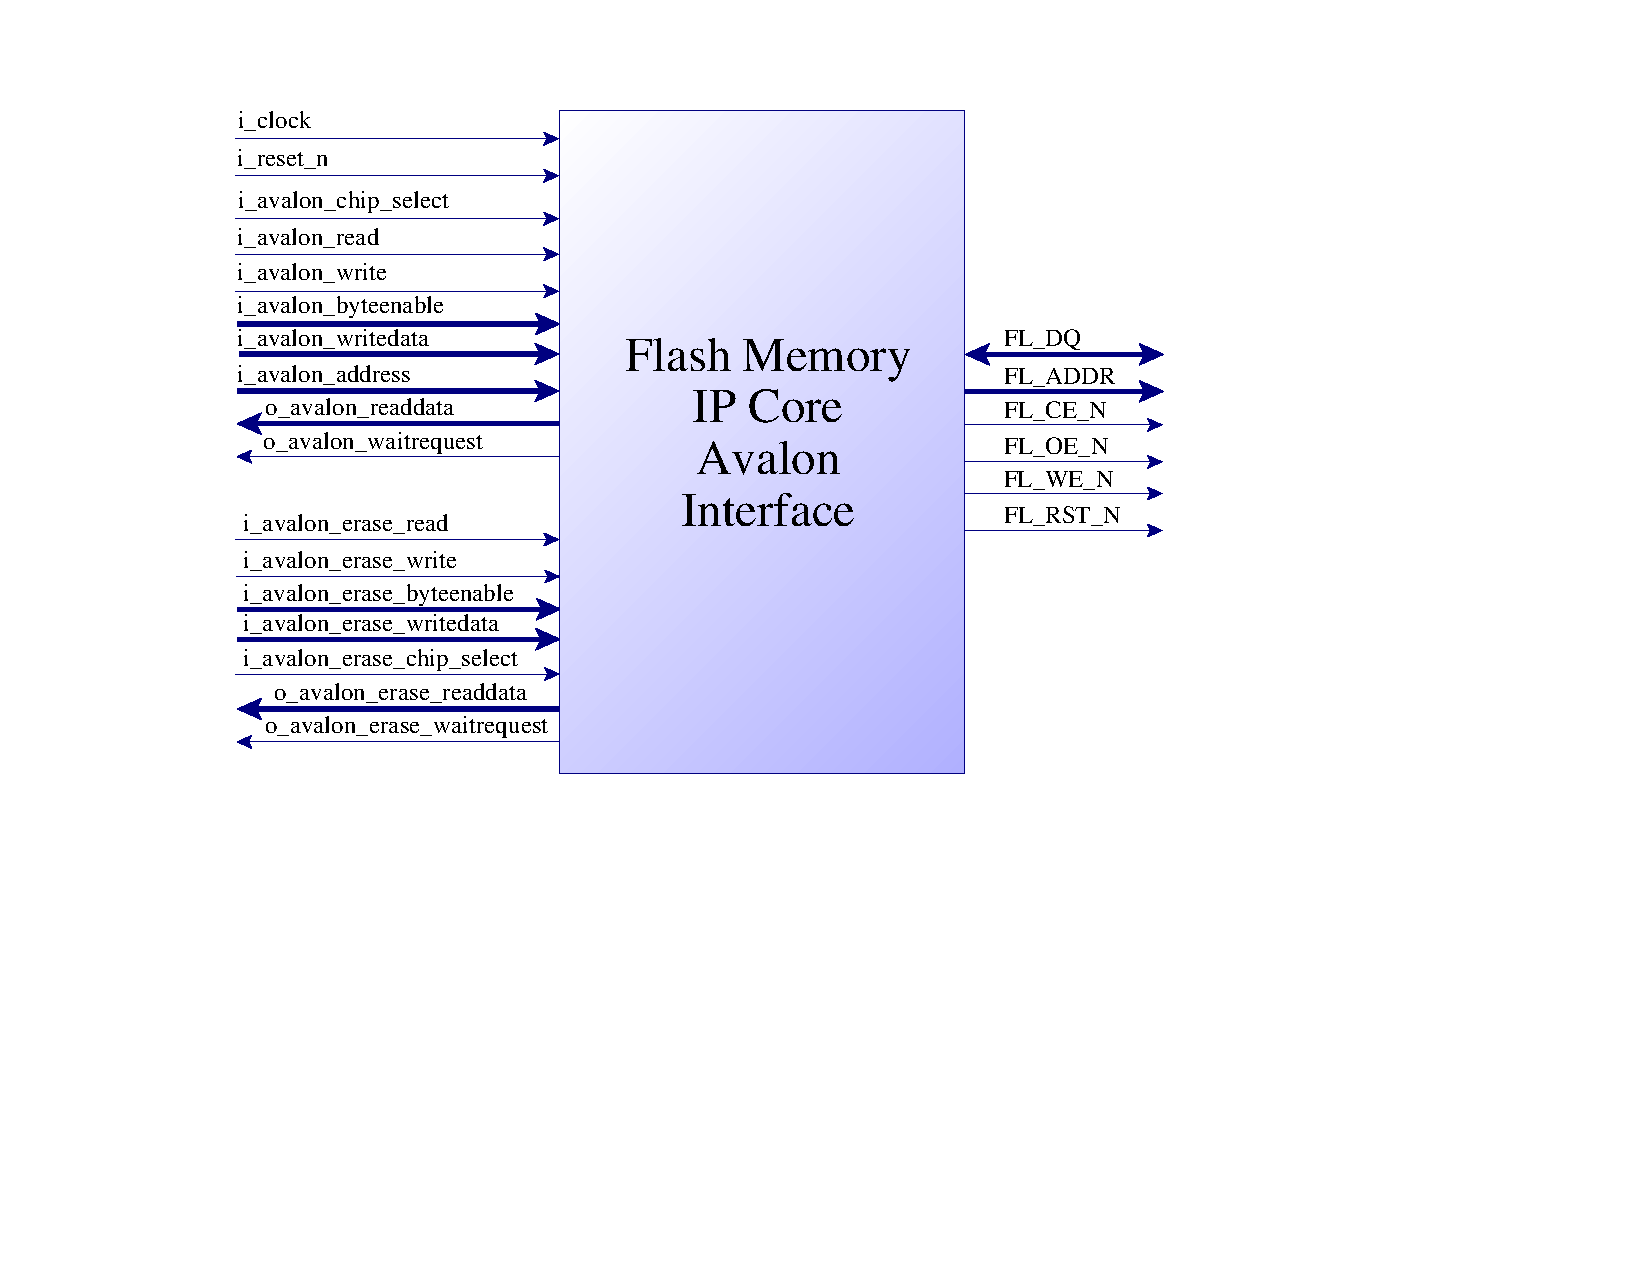
\includegraphics[width=4in,,,clip=false]{fig_flash_avalon_interface.pdf}
\caption{SOPC Builder Flash Memory IP Core with Avalon Interconnect Interface.}\label{fig:avalon_interface}
\end{figure}

This module is similar to the standalone version of the core, except in how it interfaces with a user circuit. In this case,
the interface is facilitated by the Avalon Interconnect fabric. The Avalon Interconnect fabric allows components to be attached
to a system and assigns an address range for each device on the interconnect. Thus, a Nios II soft-core processor that connects to
peripheral devices by the means of this interconnect, can access each device as a memory mapped slave, simply by providing the
appropriate address to the Avalon Interconnect.

The Altera UP Flash Memory IP Core has two memory-mapped slave ports that connect to the Avalon Interconnect. One set, allows
data to be transferred to and from flash memory. This allows the flash memory to appear as though it is a regular memory with
read and write capability. The other set, labeled {\it *\_avalon\_erase\_*} is a set of ports that provides access to an erase-control
register.

The erase-control register is a 32-bit register used to control the erasing operation of flash memory
device. Writing an address to this register causes the core to erase a sector containing the specified address. In a special case,
when the address is (-1), the entire flash memory device will be erased. Please note that while the erase operation is in progress,
the avalon interconnect will wait for the operation to complete. This means that another request to the flash memory device cannot
be issued during that time.

\section{Instantiating the Flash Memory IP Core}
\label{sec:instantiation}

To use the Altera UP Flash Memory IP Core, the core needs to be instantiated in a design. This can be done in two ways: as a standalone module that functions in a manner similar to regular memory, or as an SOPC Builder component connected to the Avalon Interconnect. Both methods of instantiating the core are described below.

\subsection{Instantiating a Standalone Version of the Core}

The Altera UP Flash Memory IP Core can be used as a standalone module that interfaces with a flash memory chip on DE boards. Users should instantiate a module called {\it Altera\_UP\_Flash\_Memory\_IP\_Core\_Standalone} to use the flash memory core in a standalone version. The input and output ports for the standalone Altera UP Flash Memory IP Core are shown in Figure~\ref{fig:standalone}, and described in detail in Section 2.

\subsection{Instantiating an SOPC Builder Version of the Core}

To include the Altera UP Flash Memory IP Core in an SOPC Builder-based design, users need to instantiate
the core using the SOPC builder tool. To do this, locate the core in the list of modules under {\sf University Program > Memory}, and click on {\sf Altera UP Flash Memory IP Core}. This will bring up a dialog box, where users will be able to specify the memory size by defining a {\it FLASH\_MEMORY\_ADDRESS\_WIDTH} parameter. By default, this parameter is set to 22, which indicates the flash memory is 4MB in size. Adjust the bitwidth according to the size of the flash memory device on your board and click Finish.

Once the core is instantiated, it is only necessary to assign an address range for
the core to use. The flash memory core has two memory mapped slave ports, each with a separate address ranges.
The first port, called {\it flash\_data}, is a port that allows reading from and writing to the flash memory.
The address range for this port matches the memory size of the flash memory chip. The second port, called {\it flash\_erase\_control}
has an address range of 4 bytes. It facilitates access to the erase-control register. Both ports should be connected to
the data master on the Avalon Interconnect.

Both of the address ranges mentioned above need to be assigned. They should be assigned such that they do not overlap with
any existing devices connected to the Avalon Interconnect fabric. Once your system is configured to include the Altera UP Flash
Memory IP Core, the generated system will contain I/O ports that need to be connected to specific pins
on the Altera DE1 or DE2 board to access the flash memory chip properly. Please refer to the specific board manual for
correct pin assignments.

\subsection{Timing Constraints}

When instantiating a Flash Memory IP core in a design it is important to set output constraints for pins that connect to the
Flash Memory chip. This is important because without such constraints signals generated by the core may arrive at the Flash
Memory chip out-of-order, thereby making the Flash Memory device appear to malfunction. For the Altera UP Flash Memory IP Core,
both the standalone and the SOPC Builder versions, the timing constraints for the $FL\_*$ signals should be set as follows:
\begin{enumerate}
\item {\it Fast Output Register} flag should be turned ON
\item $T_{co}$ requirement should be set to no more than 10ns, and
\item $T_{su}$ requirement should be set to no more than 10ns.
\end{enumerate}

% NOTE: enable this section if applicable
%\section{Simulation Considerations}

\section{Software Programming Model}
% This section describes how the core appears from a software perspective.
% Memory components typically do not have a programming model, which is OK;
% just state that the component doesn't provide any software.

The Altera UP Flash Memory IP Core has a simple interface. The memory can be accessed by reading and writing data to the
address range occupied by the Altera UP Flash Memory IP Core. This address range it occupies is specified within the SOPC
Builder software. In addition, an erase-control register that allows the flash memory to be erased is provided separately. It is
a memory-mapped register, whose location in memory is specified in the SOPC Builder based system.

The erase-control register provides a means to erase part, or all, contents of the flash memory device. To erase a portion
of the memory, write an address to the erase-control register. The Altera UP Flash Memory IP Core will take this address and
erase the sector in the flash memory that contains the specified memory location. Please note that a sector of flash memory
can be 8 or 64 kbytes in size for a 4MB flash memory devices on DE1 and DE2 boards. To erase the contents of the entire flash
memory device, write (-1) to the flash memory erase-control register.

\section{Summary}

This document described the Altera University Program Flash Memory IP Core for Altera DE1 and DE2 boards. A demonstration program
of how this core can be used, called \textit{Altera University Program Flash Memory Demo}, can be found on Altera University Program Website.								

\end{document}
